%%%%%%%%%%%%%%%%%%%%%%%%%%%%%%%%%%%%%%%%%
% Beamer Presentation
% LaTeX Template
% Version 1.0 (10/11/12)
%
% This template has been downloaded from:
% http://www.LaTeXTemplates.com
%
% License:
% CC BY-NC-SA 3.0 (http://creativecommons.org/licenses/by-nc-sa/3.0/)
%
%%%%%%%%%%%%%%%%%%%%%%%%%%%%%%%%%%%%%%%%%

%----------------------------------------------------------------------------------------
%	PACKAGES AND THEMES
%----------------------------------------------------------------------------------------

\documentclass{beamer}

\mode<presentation> {

% The Beamer class comes with a number of default slide themes
% which change the colors and layouts of slides. Below this is a list
% of all the themes, uncomment each in turn to see what they look like.

%\usetheme{default}
%\usetheme{AnnArbor}
%\usetheme{Antibes}
%\usetheme{Bergen}
%\usetheme{Berkeley}
%\usetheme{Berlin}
\usetheme{Boadilla}
%\usetheme{CambridgeUS}
%\usetheme{Copenhagen}
%\usetheme{Darmstadt}
%\usetheme{Dresden}
%\usetheme{Frankfurt}
%\usetheme{Goettingen}
%\usetheme{Hannover}
%\usetheme{Ilmenau}
%\usetheme{JuanLesPins}
%\usetheme{Luebeck}
%\usetheme{Madrid}
%\usetheme{Malmoe}
%\usetheme{Marburg}
%\usetheme{Montpellier}
%\usetheme{PaloAlto}
%\usetheme{Pittsburgh}
%\usetheme{Rochester}
%\usetheme{Singapore}
%\usetheme{Szeged}
%\usetheme{Warsaw}

% As well as themes, the Beamer class has a number of color themes
% for any slide theme. Uncomment each of these in turn to see how it
% changes the colors of your current slide theme.

%\usecolortheme{albatross}
%\usecolortheme{beaver}
%\usecolortheme{beetle}
%\usecolortheme{crane}
%\usecolortheme{dolphin}
%\usecolortheme{dove}
%\usecolortheme{fly}
%\usecolortheme{lily}
%\usecolortheme{orchid}
%\usecolortheme{rose}
%\usecolortheme{seagull}
%\usecolortheme{seahorse}
%\usecolortheme{whale}
%\usecolortheme{wolverine}

%\setbeamertemplate{footline} % To remove the footer line in all slides uncomment this line
%\setbeamertemplate{footline}[page number] % To replace the footer line in all slides with a simple slide count uncomment this line

%\setbeamertemplate{navigation symbols}{} % To remove the navigation symbols from the bottom of all slides uncomment this line
}

\usepackage{graphicx} % Allows including images
\usepackage{booktabs} % Allows the use of \toprule, \midrule and \bottomrule in tables


\usepackage[spanish, es-lcroman]{babel} % Idioma
\selectlanguage{spanish}
\usepackage{verbatim} % Para comment


\usepackage{appendix} %Para el apéndice


\usepackage{ragged2e} %para alinear texto izqda y derecha




\usepackage{mathtools}
\usepackage{amsmath} % Movidas útiles
\usepackage{amssymb} % Simbolos mates
\usepackage{amsthm} % Personalizar teoremas (mas abajo continuacion)
\usepackage{thmtools} % Mas movidas teoremas

\usepackage{tikz} % Para pictures
\usetikzlibrary{decorations.markings,arrows} %decoracion en tikz
\usetikzlibrary{shadows,arrows,positioning,shapes.geometric}
\usetikzlibrary{decorations,decorations.markings}
\usepackage{pgfplots}
\usetikzlibrary{intersections, pgfplots.fillbetween}
\usetikzlibrary {arrows.meta}

\usepackage{etoolbox}
\usetikzlibrary{optics}
\usepackage{pgf,tikz}
\usetikzlibrary{arrows}
\usetikzlibrary{babel}



%\sectionfont{\underline} % Titulo seccion subrayado

% Comandos simbolos utiles 
\newcommand{\C}{\mathbb{C}}
\newcommand{\R}{\mathbb{R}}
\newcommand{\Q}{\mathbb{Q}}
\newcommand{\Z}{\mathbb{Z}}
\newcommand{\N}{\mathbb{N}}
\newcommand{\Epsilon}{\mathcal{E}}
\DeclareMathOperator{\interior}{Int} %interior
\DeclareMathOperator{\dimension}{dim} %dimension
\DeclareMathOperator{\Ker}{Ker}
\DeclareMathOperator{\Ab}{Ab}


\newcommand{\norm}[1]{\left\lVert#1\right\rVert} % Comando para normas
\newcommand{\Esfera}{\mathbb{S}^2}
\newcommand{\Toro}{\mathbb{T}^2}
\newcommand{\Proyectivo}{\mathbb{P}^2}
\newcommand{\enfatiza}[1]{\textbf{\textit{#1}}}
\newcommand{\Disco}{\overline{\mathbb{B}}^2}
% Estilos teoremas (Mejorable)
\theoremstyle{definition}
\newtheorem{defin}{Definición}[section]
\newtheorem{tma}[defin]{Teorema}
\newtheorem*{tma*}{Teorema}
\newtheorem{corol}[defin]{Corolario}
\newtheorem{prop}[defin]{Proposición}
\newtheorem{lema}[defin]{Lema}
%\newcommand{\demo}{Demostración.\\}
%\newcommand{\ok}{\hfill$\square$}
%\theoremstyle{remark}
\newtheorem{obs}[defin]{Observación}
\newtheorem{eje}[defin]{Ejemplo}
\graphicspath{ {images/} }
\usepackage{afterpage}

\newcommand\blankpage{%
    \null
    \thispagestyle{empty}%
    \newpage}
\usepackage{caption}
\usepackage{subcaption} %para hacer subfigures

%bibliografia

\usepackage[backend=bibtex, style=numeric, sorting=none, defernumbers=true]{biblatex}
\addbibresource{bibliografiatfg.bib}




%----------------------------------------------------------------------------------------
%	TITLE PAGE
%----------------------------------------------------------------------------------------

\title[Trabajo de Fin de Grado]{La Prueba ZIP de Conway del Teorema de Clasificación de Superficies} % The short title appears at the bottom of every slide, the full title is only on the title page

\author{Juan Valero Oliet} % Your name
\institute[UCM] % Your institution as it will appear on the bottom of every slide, may be shorthand to save space
{
Universidad Complutense de Madrid \\ % Your institution for the title page
\medskip
\textit{Dirigido por: Manuel Alonso Morón} % Your email address
}
\date{\today} % Date, can be changed to a custom date

\begin{document}

\begin{frame}
\titlepage % Print the title page as the first slide
\end{frame}

%\begin{frame}
%\frametitle{Esquema} % Table of contents slide, comment this block out to remove it
%\tableofcontents % Throughout your presentation, if you choose to use \section{} and \subsection{} commands, these will automatically be printed on this slide as an overview of your presentation
%\end{frame}

%----------------------------------------------------------------------------------------
%	PRESENTATION SLIDES
%----------------------------------------------------------------------------------------

%------------------------------------------------
\section{Introducción} % Sections can be created in order to organize your presentation into discrete blocks, all sections and subsections are automatically printed in the table of contents as an overview of the talk
%------------------------------------------------

%\subsection{Subsection Example} % A subsection can be created just before a set of slides with a common theme to further break down your presentation into chunks

\begin{frame}
\frametitle{Introducción al trabajo}
 

\begin{tma}[Clasificación de Superficies]
Sea $S$ una superficie compacta y conexa. Entonces $S$ es homeomorfa a una y sólo una de las siguientes superficies: 
\begin{itemize}
\item La esfera $\Esfera$. 
\item Una suma conexa de copias del toro $\Toro \# \dots \# \Toro$. 
\item Una suma conexa de copias del plano proyectivo $\Proyectivo \# \dots \# \Proyectivo$.

\end{itemize}
\end{tma}

\frametitle{}
\begin{figure}
\centering%%%%FIG: Toro y esfera
\begin{subfigure}{.3\textwidth}
\centering
\begin{tikzpicture}[scale=0.5]
\draw (0,0) circle (2cm);
\draw (2,0) arc[x radius=2, y radius=0.7, start angle=0, end angle=-180];
\draw [dashed] (2,0) arc[x radius=2, y radius=0.7, start angle=0, end angle=180];
\end{tikzpicture}
\caption{$\Esfera$}
\end{subfigure}
\begin{subfigure}{.3\textwidth}
\centering
\begin{tikzpicture}[scale=.5]
\draw (6,-0.1) ellipse (2.9cm and 1.4 cm);
\draw (7.5,0.1) arc[x radius=1.5, y radius=0.4, start angle=0, end angle=-180];
\draw (7.3,-0.1) arc[x radius=1.3, y radius=0.3, start angle=0, end angle=180]; 
\end{tikzpicture}
\caption{$\Toro$}
\end{subfigure}	
\begin{subfigure}{0.3\textwidth}
\centering
\begin{tikzpicture} [scale=.5]


\draw [] (5,-3)-- (5,-1.5);
\draw (3,-3) arc[x radius=2, y radius=2.5, start angle=180, end angle=360];
\draw [out=90,in=360] (7,-3) to (5,-1.5);
\draw [out=180, in=90] (5, -1.5) to (3,-3);
\draw [color=gray][out=270, in=225, looseness=0.7] (3,-3) to (5,-3);
\draw [color=gray][dashed][out=45, in=90, looseness=0.7] (5,-3) to (7,-3);
\draw [color=gray][dashed][out=90, in=135, looseness=0.7] (3,-3) to (5,-3);
\draw [color=gray][out=-45, in=-90, looseness=0.7] (5,-3) to (7,-3);


%\fill [color=black] (-7,3) circle (1.5pt);
%\fill [color=black] (-5,5) circle (1.5pt);
%\fill [color=black] (-3,3) circle (1.5pt);
%\fill [color=black] (-5,1) circle (1.5pt);
%\fill [color=black] (-2,3.5) circle (1.5pt);
%\fill [color=black] (3,3.5) circle (1.5pt);
%\fill [color=black] (7,3.5) circle (1.5pt);
%\fill [color=black] (5,3.5) circle (1.5pt);
%\fill [color=black] (2,3.5) circle (1.5pt);
%\fill [color=black] (0,4) circle (1.5pt);
%\fill [color=black] (0,3) circle (1.5pt);
%\fill [color=black] (2,-3) circle (1.5pt);
%\fill [color=black] (-2,-3) circle (1.5pt);
%\fill [color=black] (0,-3) circle (1.5pt);
%\fill [color=black] (5,-1.5) circle (1.5pt);
%\fill [color=black] (5,-3) circle (1.5pt);
%\fill [color=black] (-7,-3) circle (1.5pt);
%\fill [color=black] (-5,-3) circle (1.5pt);
%\fill [color=black] (-3,-3) circle (1.5pt);

\end{tikzpicture}
\caption{$\Proyectivo$}
\end{subfigure}
\end{figure}
\end{frame}




%----
\begin{frame}
\frametitle{Introducción Histórica}
\begin{itemize}
\item 1863 - Möbius
\item 1866 - Jordan
\item 1888 - von Dick
\item 1907 - Dehn y Heegard
\item 1915 - Alexander
\item 1920 - Brahana
\item 1925 - Radó\pause
\end{itemize}

Textos de hoy en día $\longrightarrow$ Seifert - Threlfall.

\end{frame}

%-------

\begin{frame}
\frametitle{Prueba ZIP}

\begin{columns}
\column{.6\textwidth} % Left column and width
\begin{itemize}

\item 1999 $\longrightarrow$ artículo de Francis y Weeks.

\item John H. Conway (1937-2020).

\item Prueba de Irrelevancia Cero. 
\end{itemize}

\column{.35\textwidth} % Right column and width
\begin{figure}
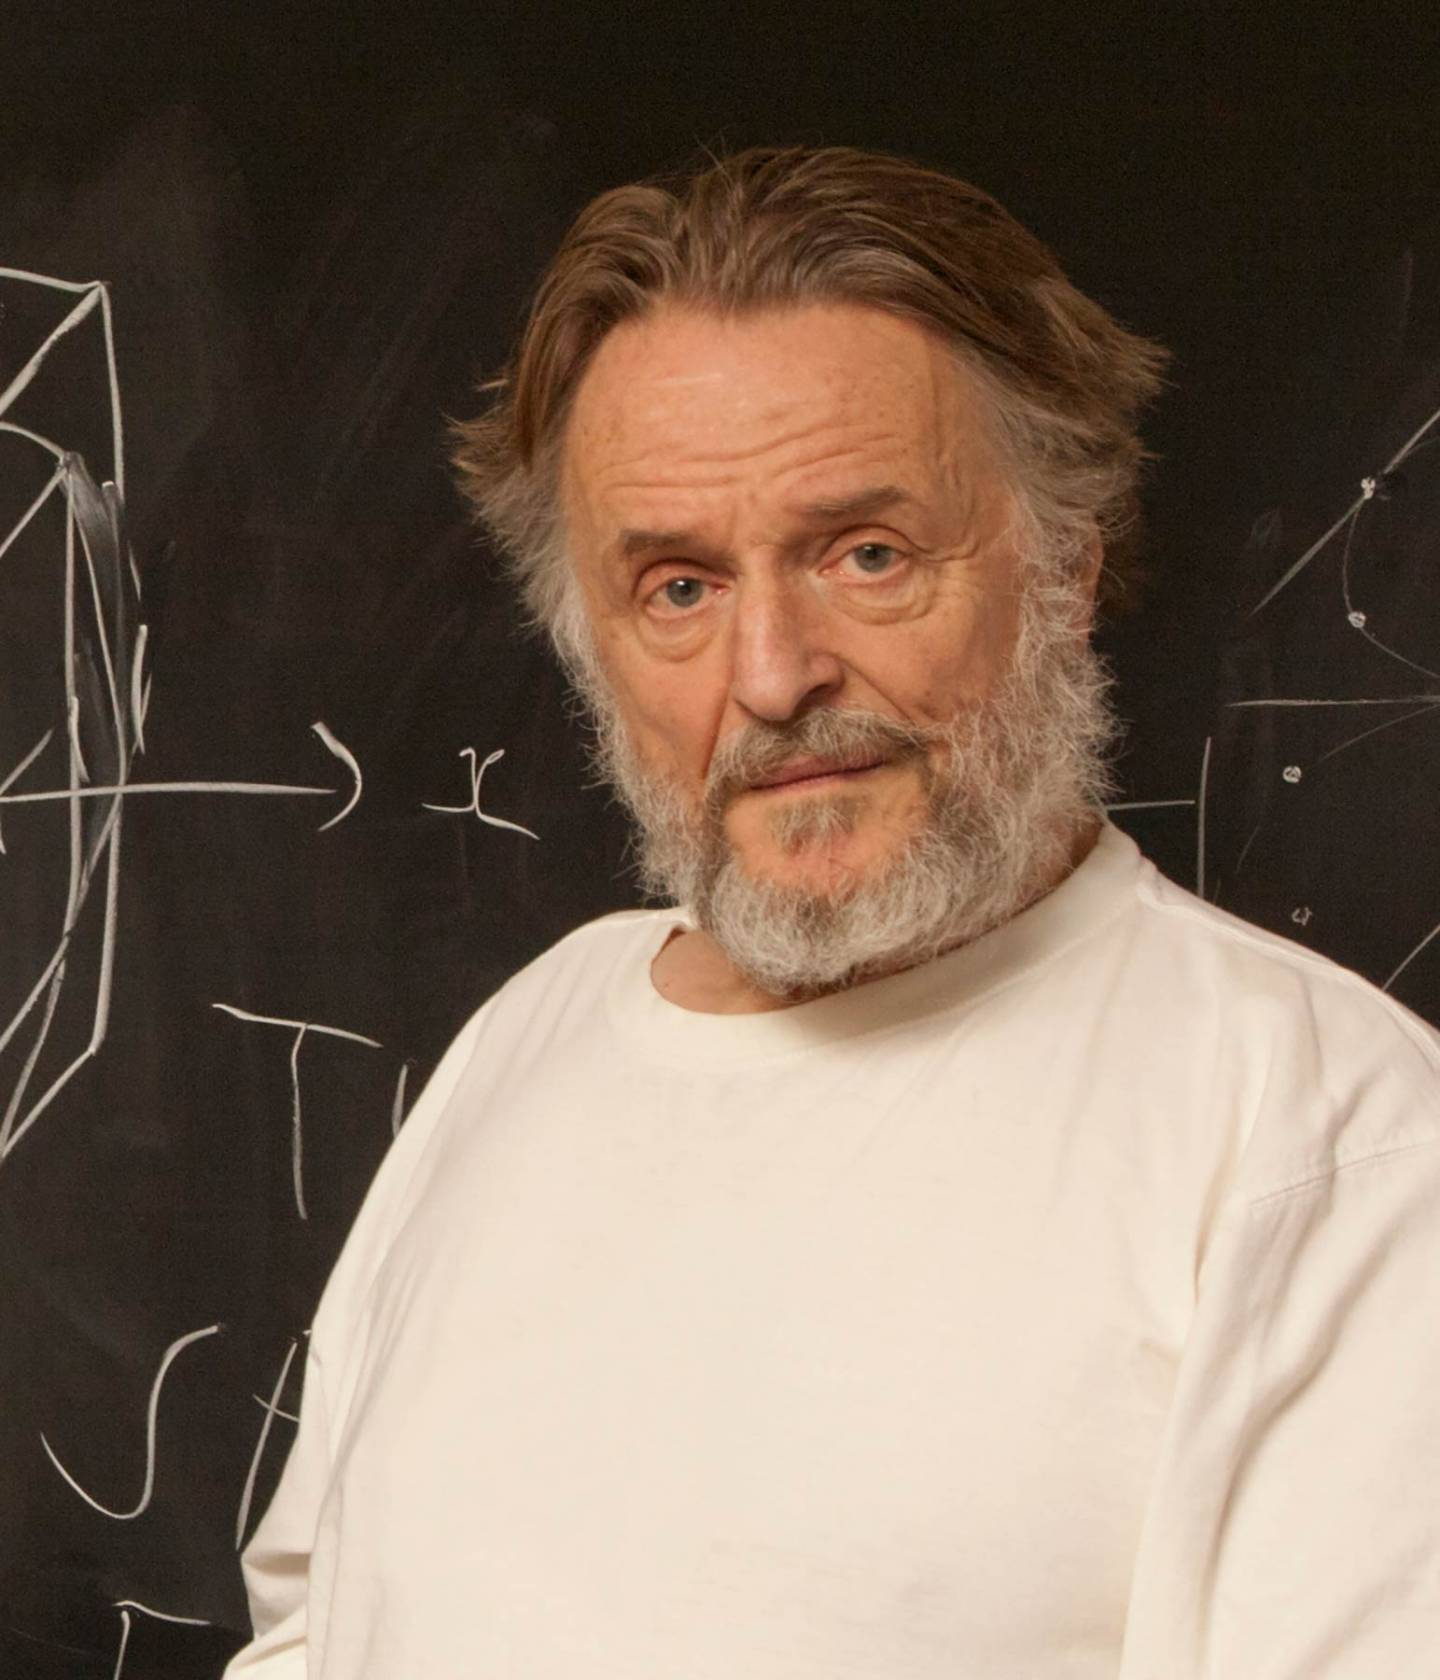
\includegraphics[scale=.07]{conway.jpg}
\end{figure}

\end{columns}

\pause

\begin{block}{Ventajas}

\begin{itemize}
\item Se basa en el concepto de suma conexa.
\item  Más intuitivo.\pause
\end{itemize}
\end{block}

\begin{block}{Problemas}

\begin{itemize}
\item No se definen algunos conceptos utilizados. 
\item No se desarrollan en profundidad algunos resultados.
\item No se demuestra que las superficies no sean homeomorfas entre sí. 
\end{itemize}
\end{block}

\end{frame}

\begin{frame}

\begin{itemize}
\frametitle{Trabajo}
\item Estudiar los conceptos previos.
\item Estudiar la demostración clásica.
\item Tratamiento riguroso de la prueba ZIP.
\item Completar con la segunda parte del teorema.
\end{itemize}
\end{frame}

\begin{frame}
\frametitle{Triangulación}

\begin{figure}
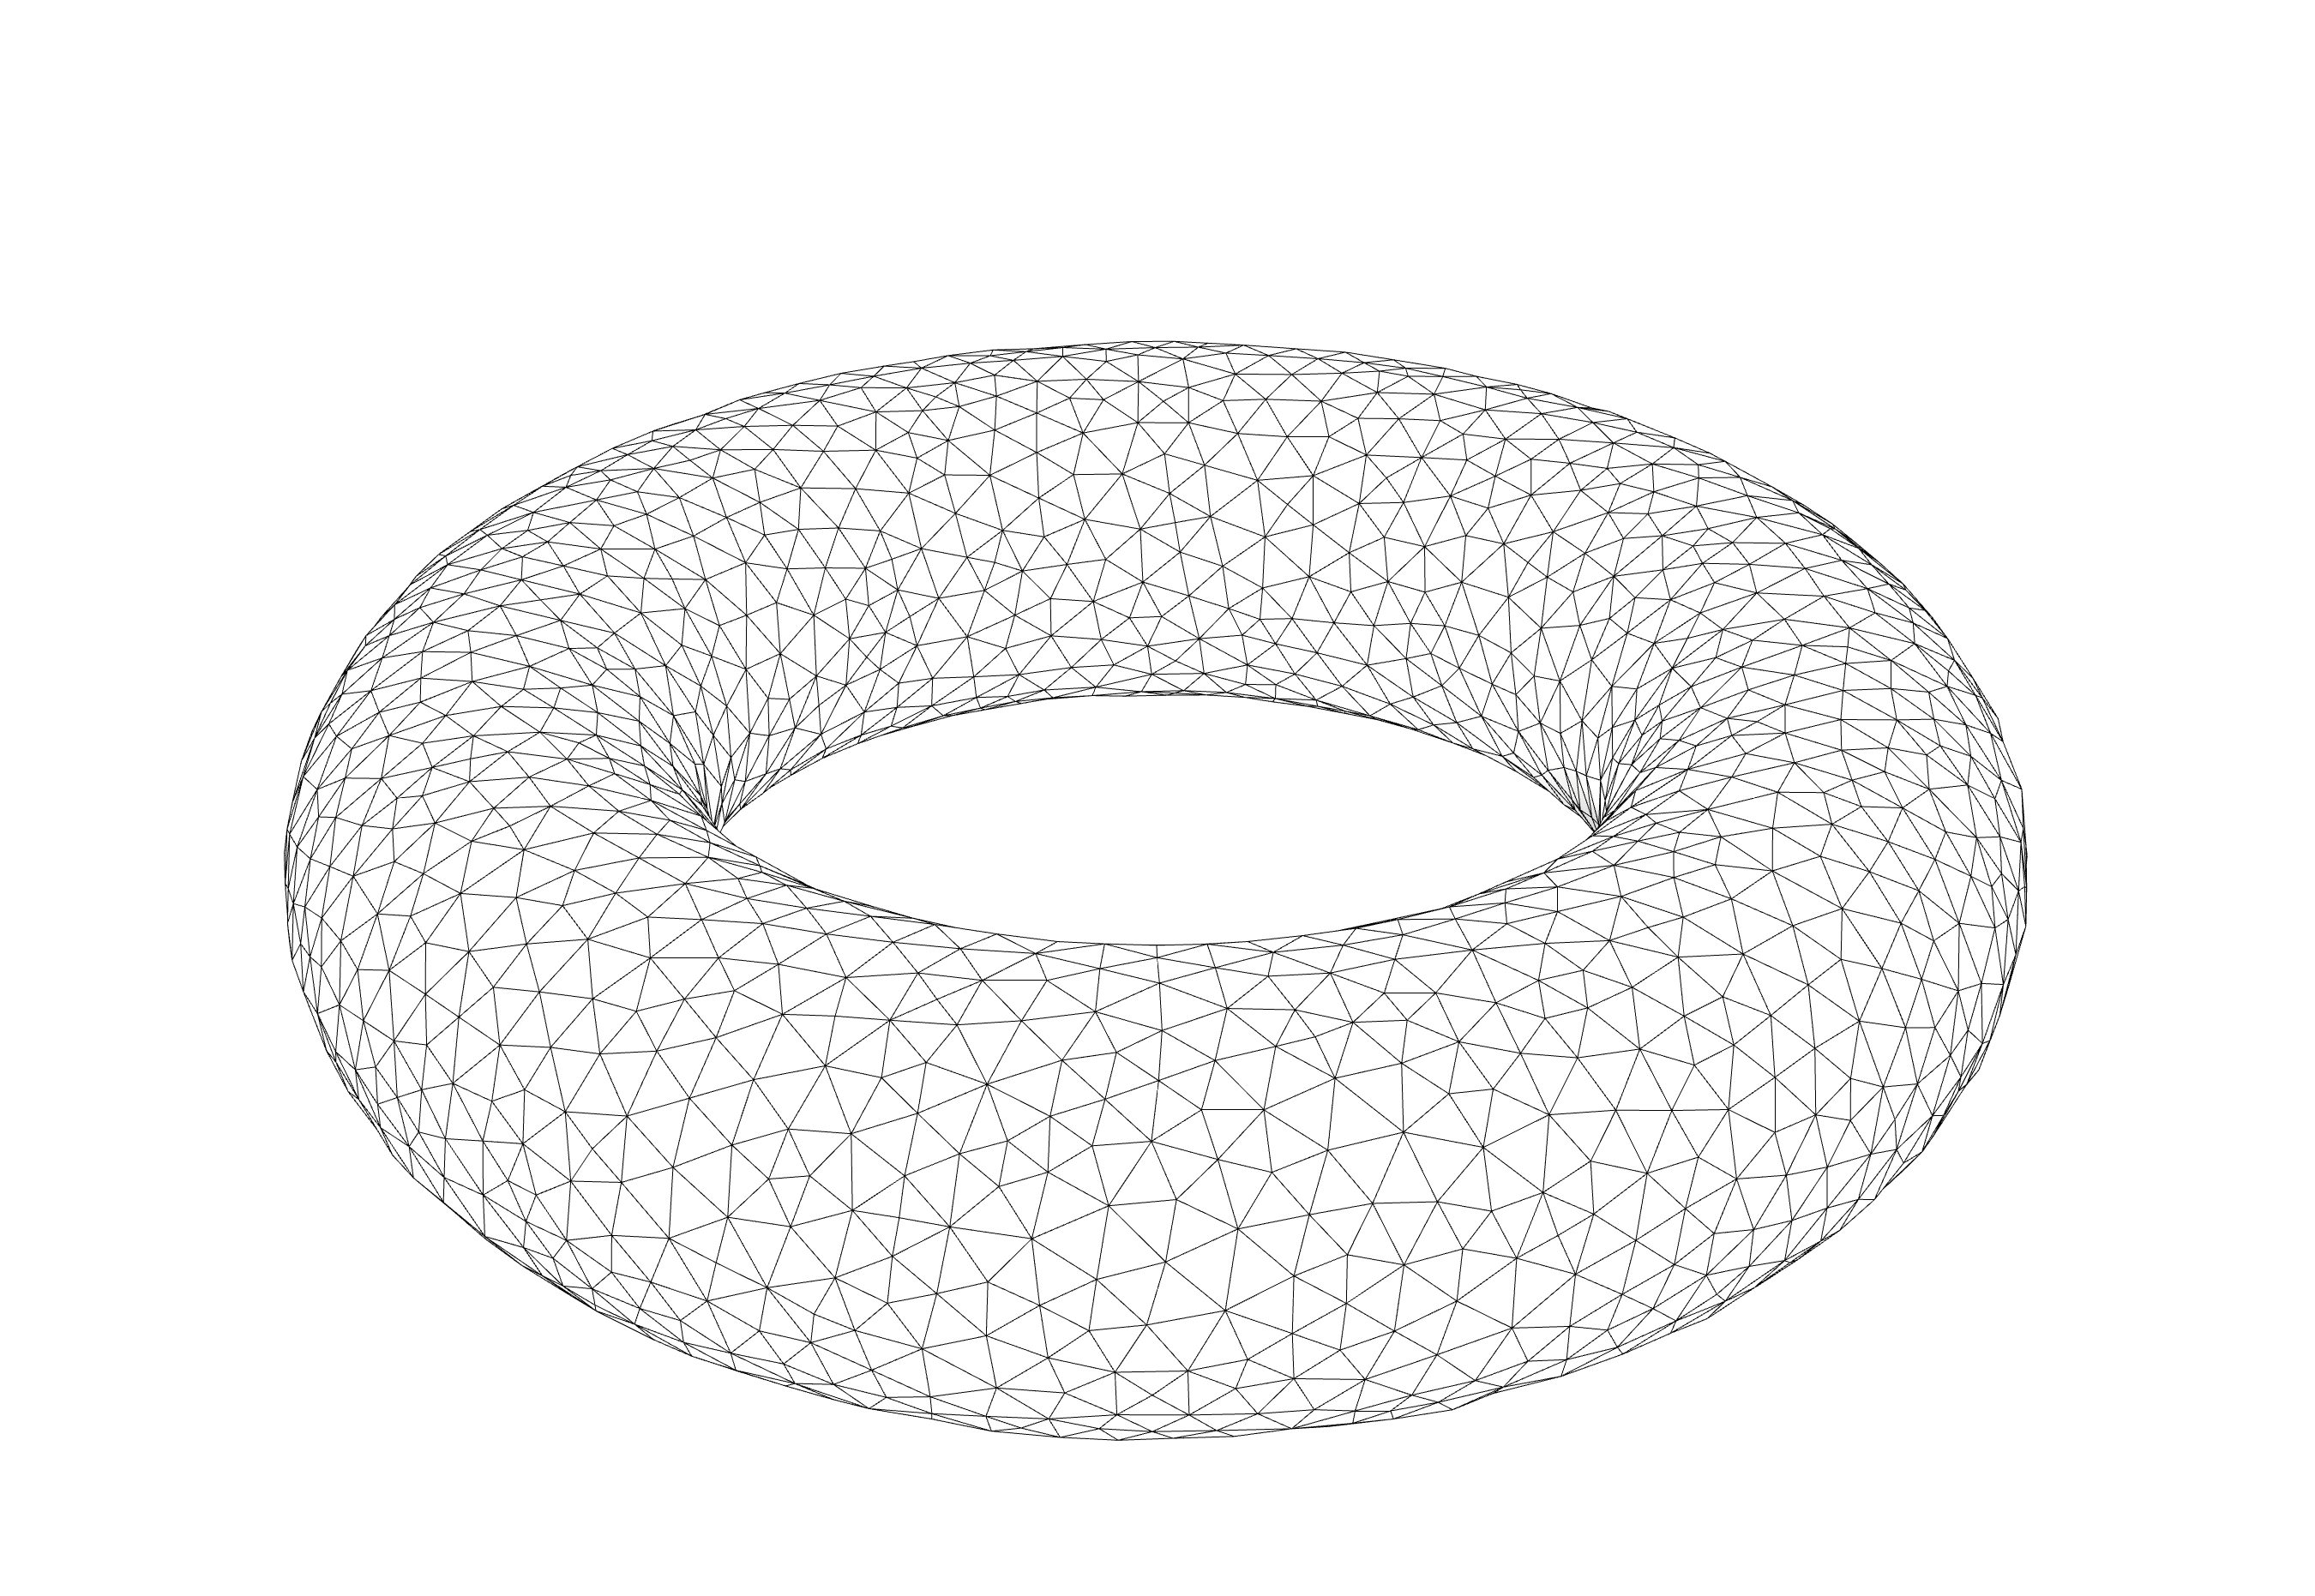
\includegraphics[scale=0.07]{./images/triangulacion.png}
\end{figure}

\begin{tma}[Teorema de Radó]
Toda superficie es triangulable.
\end{tma}

\begin{tma}[Teorema de Schönflies]
Sea $f$ un homeomorfismo entre dos curvas simples cerradas $C$ y $C'$. Entonces $f$ se puede extender a un homeomorfismo de todo el plano.
\end{tma}
\end{frame}

\begin{frame}
\frametitle{Teorema de Radó}
Idea de la demostración (Thomassen)
\begin{itemize}
\item Recubrir la superficie con un número finito de discos coordenados.
\item Triangular cada disco de forma que sea compatible con los anteriores.
\end{itemize}
%Dificultades:\pause
%\begin{itemize}
%\item Mostrar que las intersecciones entre las curvas son un número finito.\pause
%\item Mostrar que las regiones que definen estas intersecciones son homeomorfas a discos cerrados $\longrightarrow$ \textit{Schönflies}.
%\end{itemize}
\end{frame}

%------------------------------------------------


\begin{frame}
\frametitle{Perforaciones}
\begin{figure}[]%%%%FIG: Disco esfera perforada
\centering
\begin{tikzpicture}[line cap=round,line join=round,>=triangle 45,x=1.0cm,y=1.0cm]
\fill[gray!20](3,0) circle (2cm);
\fill[color=gray!20][rotate around={-14.04:(-1.34,0.02)}] (-1.34,0.02) ellipse (0.32cm and 0.24cm);
\fill[color=white][rotate around={-14.04:(3.33,1.31)}] (3.33,1.31) ellipse (0.32cm and 0.24cm);
\draw[rotate around={-14.04:(-1.34,0.02)}] (-1.34,0.02) ellipse (0.32cm and 0.24cm);
\draw[rotate around={-14.04:(3.33,1.31)}] (3.33,1.31) ellipse (0.32cm and 0.24cm);
\draw(3,0) circle (2cm);
\draw(1,0) arc[x radius=2, y radius=0.5, start angle=180, end angle=360];
\draw[dashed](5,0) arc[x radius=2, y radius=0.5, start angle=0, end angle=180];
\draw(0,0) node[anchor=north] {$ \approx $};
%\draw [out=-14.04, in=0, looseness=2] (-1.28,0.26) to (-1.5,-2);
%\draw [out=180, in=165.96, looseness=4] (-1.5,-2) to (-1.28,0.26);
\end{tikzpicture}
\caption{El disco cerrado como una esfera perforada.\label{fig:disco_esfera_perforada}}
\end{figure}
\end{frame}


\begin{frame}
\frametitle{Perforaciones}
\begin{prop}
Toda superficie con borde compacta es homeomorfa a una superficie compacta con perforaciones.
\end{prop}

\begin{prop}[Teorema de Clasificación]
Sean $M_1$ y $M_2$ superficies con borde compactas tales que $\partial M_1$ y $\partial M_2$ tienen el mismo número de componentes conexas. Entonces $M_1$ y $M_2$ son homeomorfas si y solo si las superficies $M_1^*$ y $M_2^*$  son homeomorfas.
\end{prop}
\end{frame}

\begin{frame}
\frametitle{Suma Conexa}
\begin{figure}%%%%FIG: 2-toro
\centering
\begin{tikzpicture}[scale=0.7]
\draw (0.23,1.85) arc[x radius=2, y radius=1.4, start angle=150, end angle=-150];
\draw (-0.23,1.85) arc[x radius=2, y radius=1.4, start angle=30, end angle=330];
\draw plot [smooth] coordinates { (-0.23,1.85) (0,1.67)(0.23,1.85)};
\draw plot [smooth] coordinates { (-0.23,0.45) (0,0.67)(0.23,0.45)};

\draw (-1.25,1.35) arc[x radius=0.7, y radius=0.5, start angle=0, end angle=-180];
\draw (-1.45,1) arc[x radius=0.5, y radius=0.3, start angle=0, end angle=180]; 
\draw (2.65,1.35) arc[x radius=0.7, y radius=0.5, start angle=0, end angle=-180];
\draw (2.45,1) arc[x radius=0.5, y radius=0.3, start angle=0, end angle=180]; 

\draw (0,1.67) arc[x radius=0.1, y radius=0.5, start angle=90, end angle=270];
\draw [dashed] (0,1.67) arc[x radius=0.1, y radius=0.5, start angle=90, end angle=-90];
\end{tikzpicture}
\caption{Suma conexa de dos toros.}
\end{figure}

\begin{enumerate}
\item Se consideran dos superficies $M_1$ y $M_2$. 
\item Realizamos una perforación en cada superficie $\longrightarrow$ superficies con borde $M_1^o$ y $M_2^o$.
\item Consideramos un homeomorfismo $f:\partial M_1^o \to \partial M_2^o$.
\item Relacionamos en $M_1^o\amalg M_2^o$ cada punto de $\partial M_1^o$ con su imagen por $f$.
\item Al espacio cociente $M=\frac{M_1^o\amalg M_2^o}{\sim}$ lo llamamos \enfatiza{suma conexa} de $M_1$ y $M_2$.
\end{enumerate}
\end{frame}
%------------------------------------------------

\begin{frame}
\frametitle{Representación de superficies}
\begin{itemize}
\item Polígonos con aristas que se identifican.
\end{itemize}

\begin{figure}[]%%%%FIGURA: TORO COMO CUADRADO
\begin{center}
\begin{tikzpicture}[use optics, line cap=round,line join=round,>=triangle 45,x=1cm, y=1cm, scale=0.5]

\draw [->-={at=0.5}](-8,-2)-- (-8,2);
\draw [->>-={at=0.5}](-8,2)-- (-4,2);
\draw [-<-={at=0.5}](-4,2)-- (-4,-2);
\draw [->>-={at=0.5}](-8,-2)-- (-4,-2);
\draw (-2,1)-- (2,1);
%\draw (-2,1)-- (-2,-1);
%\draw (2,1)-- (2,-1);
\draw (2,-1)-- (-2,-1);
%\draw [-<-={at=0.6]}](2,1) arc[x radius=0.5, y radius=1, start angle=90, end angle=270];
%\draw (2,1) arc[x radius=0.5, y radius=1, start angle=90, end angle=-90];
\draw [-<-={at=0.6]}](-2,1) arc[x radius=0.5, y radius=1, start angle=90, end angle=270];
\draw [dashed] (-2,1) arc[x radius=0.5, y radius=1, start angle=90, end angle=-90];
\filldraw [-<-={at=0.55]}][color=black, fill=black!0] [rotate around={0:(2,0)}] (2,0) ellipse (0.5cm and 1cm);
\draw [->>-={at=0.5}](-2.5,0)-- (1.5,0);
\draw [rotate around={0:(6,0)}] (6,0) ellipse (3cm and 1.5cm);
\draw (7.4,0.1) arc[x radius=1.5, y radius=0.4, start angle=0, end angle=-180];
\draw (7.2,-0.1) arc[x radius=1.3, y radius=0.3, start angle=0, end angle=180]; 
\draw [dashed](6,-1.5) arc[x radius=0.2, y radius=0.6, start angle=-90, end angle=90];
\draw [-<-={at=0.63}] (6,-0.3) arc[x radius=0.2, y radius=0.6, start angle=90, end angle=270];
\begin{scriptsize}
\fill [color=black] (-8,-2) circle (1.5pt);
\fill [color=black] (-8,2) circle (1.5pt);
\fill [color=black] (-4,2) circle (1.5pt);
\fill [color=black] (-4,-2) circle (1.5pt);
\fill [color=black] (-2.5,0) circle (1.5pt);
\fill [color=black] (1.5,0) circle (1.5pt);
\fill [color=black] (5.8,-0.9) circle (1.5pt);
\end{scriptsize}
\end{tikzpicture}
\end{center}
\caption{El toro como cociente de un cuadrado.\label{fig:toro_cuadrado}}
\end{figure}
\end{frame}

\begin{frame}
\frametitle{Representación de superficies}

\begin{figure}%%%%FIG: Klein
\centering
\begin{tikzpicture} [use optics]
%\draw [help lines] (-6,-2) grid (6,2);
%1
\draw[-<<-={at=0.125}, -<-={at=0.375}, ->>-={at=0.625}, -<-={at=0.875}] (-5,-1) -- (-5,1) -- (-3,1) -- (-3, -1) -- (-5,-1);
%2
\draw[-<<-] (-1.7, -1.085)--+(0,2);
\draw [-<-={at=0.43}, -<-={at=0.897}] (-2,-1) -- +(0,2) arc[x radius=0.5, y radius=0.1, start angle=180, end angle=360] -- +(0,-2) arc[x radius=0.5, y radius=0.1, start angle=0, end angle=-180];
\draw [dashed] (-2,-1) arc[x radius=0.5, y radius=0.1, start angle=180, end angle=0];
\draw (-2,1) arc[x radius=0.5, y radius=0.1, start angle=180, end angle=0];
%3
\draw [->-={at=0.535}, ->-={at=0.974}](0.2,-0.5) [out=80, in=180] to (1.64,1.5) [out=0, in=100] to (3,-1) arc [x radius=0.35, y radius=0.1, start angle=0, end angle=-180] [out=85, in=0] to (1.64,1) [out=180, in=95] to (0.75, -0.5) arc[x radius=0.275, y radius=0.1, start angle=0, end angle=-180];
\draw [dashed] (0.2,-0.5) arc[x radius=0.275, y radius=0.1, start angle=180, end angle=0] (3,-1) arc[x radius=0.35, y radius=0.1, start angle=0, end angle=180];

%4
\draw [->-={at=0.07}][dash pattern= on 52.5pt off 2pt on 2pt off 2pt on 2pt off 2pt on 79.5pt off 2pt on 2pt off 2pt on 2pt off 2pt on 2pt off 2pt on 2pt off 2pt on 2.2pt off 2pt on 2pt off 2pt on 2pt off 2pt on 2pt off 2pt on 2pt off 2pt on 2pt off 2pt on 200pt]
	(5,-1) arc[x radius=0.4, y radius=0.1, start angle=0, end angle=-180] [out=135, in= 270] to +(-0.2,0.6) [out=90, in=270] to +(0.5,1) [out=90, in=0] to (4.3,1) [out=180, in=90] to +(-0.2,-0.3) [out=270, in=135] to +(0.5, -0.8) [out=-65, in=-65] to +(-0.3,-0.2) [out=-80, in=80] to (4.2,-1) arc [x radius=0.4, y radius=0.1, start angle=180, end angle=0] ;

\draw [dash pattern= on 2pt off 2pt on 2pt off 2pt on 2pt off 2pt on 2pt off 2pt on 2pt off 2pt on 2pt off 2pt on 2pt off 2pt on 2pt off 2pt on 2pt off 2pt on 2pt off 2pt on 180pt ](5,-1)[out=100, in=-45] to (4.6,-0.1) [out=115, in=115] to +(-0.3,-0.2) [out=135, in=270] to +(-0.5,1) [out=90, in=180] to (4.4,1.3) [out=0, in=90] to +(0.4, -0.7) [out=-90, in=90] to +(0.4,-1) [out=-90, in=45] to (5,-1);


\draw [-Stealth](-.4,1.5) arc[x radius=0.4, y radius=0.2, start angle=150, end angle=30];
\draw [-Stealth](-2.8,1.5) arc[x radius=0.4, y radius=0.2, start angle=150, end angle=30];
\draw [-Stealth](3,1.5) arc[x radius=0.4, y radius=0.2, start angle=150, end angle=30];
\end{tikzpicture}
\caption{Construcción de la botella de Klein.\label{fig:klein}}
\end{figure}
\end{frame}



\begin{frame}
\frametitle{Representación de superficies}
\begin{figure}[]%%%%FIG: Representación de superficies impoirtantes
\centering
\begin{subfigure}{0.3\textwidth}
\centering
\begin{tikzpicture}[use optics, line cap=round,line join=round,>=triangle 45,x=1.0cm,y=1.0cm, scale=0.5]
\draw [-<-](0,2)-- (2,0);
\draw [-<-](2,0)-- (0,-2);
\draw [-<-](0,-2)-- (-2,0);
\draw [-<-](-2,0)-- (0,2);
\draw (1,1) node[anchor=south west] {$ b $};
\draw (1,-1) node[anchor=north west] {$ a $};
\draw (-1,1) node[anchor=south east] {$ a $};
\draw (-1,-1) node[anchor=north east] {$ b $};
\end{tikzpicture}
\caption{El plano proyectivo $\Proyectivo$.}
\end{subfigure}
\begin{subfigure}{0.3\textwidth}
\centering
\begin{tikzpicture}[use optics, line cap=round,line join=round,>=triangle 45,x=1.0cm,y=1.0cm, scale=0.5]
\draw [-<-](3,0)-- (5,2);
\draw [->-](5,2)-- (7,0);
\draw [->-](7,0)-- (5,-2);
\draw [-<-](5,-2)-- (3,0);
\draw (6,1) node[anchor=south west] {$ b $};
\draw (6,-1) node[anchor=north west] {$ a $};
\draw (4,1) node[anchor=south east] {$ a $};
\draw (4,-1) node[anchor=north east] {$ b $};
\end{tikzpicture}
\caption{El toro $\Toro$.}
\end{subfigure}
\begin{subfigure}{0.3\textwidth}
\centering
\begin{tikzpicture}[use optics, line cap=round,line join=round,>=triangle 45,x=1.0cm,y=1.0cm, scale=0.5]
\draw [-<-](-3,0)-- (-5,2);
\draw [-<-](-5,-2)-- (-3,0);
\draw [-<-](-5,-2)-- (-7,0);
\draw [-<-](-7,0)-- (-5,2);
\draw (-4,1) node[anchor=south west] {$ a $};
\draw (-4,-1) node[anchor=north west] {$ b $};
\draw (-6,1) node[anchor=south east] {$ a $};
\draw (-6,-1) node[anchor=north east] {$ b $};
\end{tikzpicture}
\caption{La esfera $\Esfera$.}
\end{subfigure}
%\caption{Representación de superficies importantes.\label{fig:Representacion_superficies_importantes}}
\end{figure}
\begin{itemize}
\item[(a)] $\mathbb{P}^2= \langle a,b\mid abab \rangle$.
\item[(b)] $\Toro=\langle a,b\mid aba^{-1}b^{-1}\rangle$.
\item[(c)] $\mathbb{S}^2=\langle a,b\mid  abb^{-1}a^{-1}\rangle$ .
\end{itemize}
\end{frame}

\begin{frame}
\frametitle{Representación de superficies con borde}

\begin{figure}[]
%\centering
\begin{subfigure}{.45\textwidth}
\centering
\begin{tikzpicture}[use optics, >=angle 60, scale=1]
\begin{scriptsize}


\fill[  ,fill=gray!20] (0,0) -- (0.9238207149966959,0.3828253995531037) -- (1.3063621711370152,1.3067637277623212) -- (0.9235367715839117,2.230584442759017) -- (-0.00040155662530578324,2.6131258988993364) -- (-0.9242222716220017,2.230300499346233) -- (-1.3067637277623212,1.3063621711370155) -- (-0.9239383282092178,0.38254145614031965) -- cycle;

\draw  [->-]  (0,0) -- (0.9238207149966959,0.3828253995531037)node[midway,below] {$b_2$};
\draw  [->-](0.9238207149966959,0.3828253995531037)-- (1.3063621711370152,1.3067637277623212)node[midway, anchor=west] {$a_2$};
\draw  [-<-](1.3063621711370152,1.3067637277623212)-- (0.9235367715839117,2.230584442759017)node[midway,anchor=west] {$b_2$};
\draw  [-<-](0.9235367715839117,2.230584442759017)-- (-0.00040155662530578324,2.6131258988993364)node[midway,anchor=south west] {$a_2$};
\draw  [->-](-0.00040155662530578324,2.6131258988993364)-- (-0.9242222716220017,2.230300499346233)node[midway,anchor=south east] {$b_1$};
\draw  [->-](-0.9242222716220017,2.230300499346233)-- (-1.3067637277623212,1.3063621711370155)node[midway,anchor=east] {$a_1$};
\draw  [-<-](-1.3067637277623212,1.3063621711370155)-- (-0.9239383282092178,0.38254145614031965)node[midway,anchor=east] {$b_1$};
\draw  [-<-](-0.9239383282092178,0.38254145614031965)-- (0,0)node[midway,below] {$a_1$};
\draw  [-<-](0,0)-- (-0.5128819104663424,1.2073243438172108) node [midway, anchor=east] {$c_1$};
\draw  [-<-](0,0)-- (0.4909162594319499,1.202150126446601)node [midway, anchor=west] {$c_2$};

\filldraw[white]  (-0.5,1.5)circle (0.2929590130705814cm);
\filldraw [white] (0.5,1.5) circle (0.2979883580250803cm);
\draw  [->-={at=0.25}](-0.5,1.5) circle (0.2929590130705814cm);
\draw  [->-={at=0.25}](0.5,1.5) circle (0.2979883580250803cm);
\draw (-0.27,1.5) node [anchor=east] {$B_1$};
\draw (0.27,1.5) node [anchor=west] {$B_2$};

\filldraw (0,0) circle (1pt);
\end{scriptsize}
\end{tikzpicture}
\caption{ }
\end{subfigure}
\begin{subfigure}{.45\textwidth}
\centering
\begin{tikzpicture}[use optics,scale=1]

\begin{scriptsize}


\fill[  fill=gray!20] (0,0) -- (0.6,0) -- (1.1405813207414512,0.2603302434705348) -- (1.5146752018566914,0.7294291329513525) -- (1.6481877622304801,1.3143858802604464) -- (1.5146752018566916,1.8993426275695406) -- (1.1405813207414515,2.3684415170503583) -- (0.6,2.6287717605208933) -- (0,2.628771760520894) -- (-0.5405813207414512,2.3684415170503588) -- (-0.9146752018566913,1.899342627569541) -- (-1.0481877622304798,1.314385880260447) -- (-0.9146752018566915,0.7294291329513529) -- (-0.5405813207414516,0.260330243470535) -- cycle;


\draw [ -<- ] (0,0)-- (0.6,0) node [anchor=north, midway] {$c_1$};
\draw [ -<- ] (0.6,0)-- (1.1405813207414512,0.2603302434705348)node [anchor=north, midway] {$B_1$};
\draw [ ->- ] (1.1405813207414512,0.2603302434705348)-- (1.5146752018566914,0.7294291329513525) node [anchor=north west, midway] {$c_1$};
\draw [ -<- ] (1.5146752018566914,0.7294291329513525)-- (1.6481877622304801,1.3143858802604464) node [midway, anchor=west] {$c_2$};
\draw [ -<- ] (1.6481877622304801,1.3143858802604464)-- (1.5146752018566916,1.8993426275695406) node [midway, anchor=west] {$B_2$};
\draw [ ->- ] (1.5146752018566916,1.8993426275695406)-- (1.1405813207414515,2.3684415170503583) node [anchor=south west, midway]  {$c_2$};
\draw [ ->- ] (1.1405813207414515,2.3684415170503583)-- (0.6,2.6287717605208933)node [midway, anchor=south] {$b_2$};
\draw [  ->-] (0.6,2.6287717605208933)-- (0,2.628771760520894)node [midway, anchor=south] {$a_2$};
\draw [ -<- ] (0,2.628771760520894)-- (-0.5405813207414512,2.3684415170503588)node [midway, anchor=south] {$b_2$};
\draw [ -<- ] (-0.5405813207414512,2.3684415170503588)-- (-0.9146752018566913,1.899342627569541)node [anchor= south east, midway] {$a_2$};
\draw [ ->- ] (-0.9146752018566913,1.899342627569541)-- (-1.0481877622304798,1.314385880260447)node [midway, anchor=east]{$b_1$};
\draw [ ->- ] (-1.0481877622304798,1.314385880260447)-- (-0.9146752018566915,0.7294291329513529) node [anchor=east, midway] {$a_1$};
\draw [  -<-] (-0.9146752018566915,0.7294291329513529)-- (-0.5405813207414516,0.260330243470535) node [anchor=north east, midway]{$b_1$};
\draw [ -<- ] (-0.5405813207414516,0.260330243470535)-- (0,0)node [anchor=north, midway] {$a_1$};

\filldraw (0,0) circle (1pt);
\filldraw (1.1405813207414515,2.3684415170503583)  circle (1pt);
\end{scriptsize}

\end{tikzpicture}
\caption{ }
\end{subfigure}
\caption{La superficie $\Toro \# \Toro$  con dos perforaciones.\label{fig:toro_perforado}}
\end{figure}

%$$\langle a_1,a_2, b_1,b_2, c_1,c_2, B_1,B_2\mid a_1b_1a_1^{-1}b_1^{-1}a_2b_2a_2^{-1}b_2^{-1}c_1B_1c_1^{-1}c_2B_2c_2^{-1}\rangle$$ 
\end{frame}

\begin{frame}
\frametitle{Operaciones elementales}

Transformaciones sobre los polígonos que den lugar a superficies homeomorfas.
\begin{figure}
\begin{subfigure}{0.45\textwidth}


\centering
\begin{tikzpicture}[use optics, x=1cm, y=1cm, scale=0.6]
\begin{scriptsize}
\draw [->-={at=0.125}, ->-={at=0.375}, -<-={at=0.625}, -<-={at=0.875}](-1,1) -- (-1,-1) -- (-3,-1) -- (-3, 1) -- (-1,1); 
\draw [->-] (1,0)-- (1.57,-1);
\draw [-<-] (1.57,-1)-- (2.73,-1);
\draw [-<-] (2.73,-1)-- (3.31,0);
\draw [-<-] (3.31,0)-- (2.73,1);
\draw [->-] (2.73,1)-- (1.58,1);
\draw [->-] (1.58,1)-- (1,0);

\draw [<->] (-.1,0)--+(0.5,0);
\draw (-0.9,0) node[anchor= west] {$ a $};
\draw (-3.1,0) node[anchor= east] {$ a $};
\draw (-2,1.1) node[anchor= south] {$ b $};
\draw (-2,-1.1) node[anchor= north] {$ b $};
\draw (2.16,1.1) node[anchor= south] {$ b $};

\draw (3.02,0.5) node[anchor= south west] {$ a $};
\draw (3.02,-0.5) node[anchor= north west] {$ e $};

\draw (2.15, -1.1) node[anchor= north] {$ b $};

\draw (1.29,-0.5) node[anchor= north east] {$ e $};
\draw (1.29,0.5) node[anchor= south east] {$ a $};
\end{scriptsize}

\end{tikzpicture}
\caption{Subdividir/Consolidar}
\end{subfigure}

\end{figure}
\end{frame}

\begin{frame}
\frametitle{Operaciones elementales}
\begin{figure}[]%%%%FIG: ejemplo operacion
\begin{subfigure}{0.45\textwidth}
\centering
\begin{tikzpicture}[use optics, scale=.8]
\begin{scriptsize}

\draw [->-] (-2.15,0.84) -- (-2.71,0.47);
\draw [->-] (-2.71,0.47)--(-3.03,-.35);
\draw [-<-] (-3.03,-.35) -- (-1.67, -0.76);
\draw [-<-] (-1.67, -0.76) -- (-1.46,0.29);
\draw [->-] (-1.46,0.29) -- (-2.15,0.84);

\draw [->-] (2.15,0.84) -- (2.71,0.47);
\draw [->-] (2.71,0.47)--(3.03,-.35);
\draw [-<-] (3.03,-.35) -- (1.67, -0.76);
\draw [-<-] (1.67, -0.76) -- (1.46,0.29);
\draw [->-] (1.46,0.29) -- (2.15,0.84);

\draw (-2.42,0.66) node[anchor=south east] {$a$};
\draw (-2.87,0.06) node [anchor=east] {$b$};
\draw (-2.35,-0.56) node[anchor= north east] {$c$};
\draw (-1.56,-.24) node [anchor= west] {$d$};
\draw (-1.81,.57) node [anchor= south west] {$e$};
\draw (2.42,0.66) node[anchor=south west] {$a$};
\draw (2.87,0.06) node [anchor=west] {$b$};
\draw (2.35,-0.56) node[anchor= north west] {$c$};
\draw (1.56,-.24) node [anchor= east] {$d$};
\draw (1.81,.57) node [anchor= south east] {$e$};

\draw [<->] (-0.25,0)--+(.5,0);
\end{scriptsize}
\end{tikzpicture}
\caption{Reflejar}
\end{subfigure} 
\begin{subfigure}{.45\textwidth}
\centering
\begin{tikzpicture}[use optics, scale=0.8]
\begin{scriptsize}

\draw [->-] (-2.15,0.84) -- (-2.71,0.47);
\draw [->-] (-2.71,0.47)--(-3.03,-.35);
\draw [-<-] (-3.03,-.35) -- (-1.67, -0.76);
\draw [-<-] (-1.67, -0.76) -- (-1.46,0.29);
\draw [->-] (-1.46,0.29) -- (-2.15,0.84);

\draw [-<-](1.67,.76)--(1.46,-.29);
\draw [->-](1.46,-.29) -- (2.15,-.84);
\draw [->-](2.15,-.84)--(2.71,-.47);
\draw [->-](2.71,-.47)--(3.03,.35);
\draw [-<-](3.03,.35)--(1.67,.76);

\draw [<->] (-0.25,0)--+(.5,0);

\draw (-2.42,0.66) node[anchor=south east] {$a$};
\draw (-2.87,0.06) node [anchor=east] {$b$};
\draw (-2.35,-0.56) node[anchor= north east] {$c$};
\draw (-1.56,-.24) node [anchor= west] {$d$};
\draw (-1.81,.57) node [anchor= south west] {$e$};

\draw (2.43035, -0.65644) node[anchor=north west] {$a$};
\draw (2.86796, -0.05807) node [anchor=west] {$b$};
\draw (2.34997, 0.55816) node[anchor= south west] {$c$};
\draw (1.56406, 0.23665) node [anchor= east] {$d$};
\draw (1.80519, -0.56713) node [anchor= north east] {$e$};
\end{scriptsize}
\end{tikzpicture}
\caption{Rotar}
\end{subfigure}

\begin{subfigure}{0.45\textwidth}
\centering
\begin{tikzpicture}[use optics, scale=0.25]
\begin{scriptsize}

\draw [<->] (-.5,0)--(.5,0);
\draw (-4.79,4.04)--(-6.79,3.04)--(-6.79,-2.96)--(-4.79,-3.96)--(-3,0)--cycle;
\draw[dashed] (-4.79,-3.96)--(-4.79, 4.04);
\draw[->-={at=0.775}] (5,4)--(3,3)--(3,-3)--(5,-4)-- cycle; 
\draw[-<-={at=0.249}] (7,4)--(7,-4)--(8.79,-0) --cycle;
\draw (-6.79,0) node[anchor=east] {$W_1$}; 
\draw (-3,0) node[anchor=west]{$W_2$};
\draw (3,0) node[anchor=east] {$W_1$};
\draw (5,0.8) node[anchor=west] {$e$};
\draw (7,-1) node[anchor=east] {$e$};
\draw (8.79,0) node[anchor=west] {$W_2$};
\end{scriptsize}
\end{tikzpicture}
\caption{Cortar/Pegar}
\end{subfigure}
\begin{subfigure}{0.45\textwidth}
\centering
\begin{tikzpicture}[use optics, scale=.8]
\begin{scriptsize}
\draw [->-](0.5, 1.53884)--(-0.30902, 0.95106);
\draw [->-](-0.30902, 0.95106)--(0,0);
\draw [->-](0,0)--(1,0);
\draw [->-](1,0)--(1.30902, 0.95106);
\draw [-<-](1.30902, 0.95106)--(0.5, 1.53884);
\draw [->-](3.11256, 0)--(4.88896, 0.000);
\draw [->-](4.88896, 0.000)--(4, 1.53884);
\draw [->-](4, 1.53884)--(3.11256, 0);
\draw [->-](4,1.54)--(4,.5);
\draw (0.1,1.24) node[anchor=south east] {$a$};
\draw (-.15, 0.48) node[anchor=north east] {$b$};
\draw (.5,0) node[anchor=north] {$c$};
\draw (1.15,0.48) node [anchor=north west] {$e$};
\draw (.9, 1.24) node [anchor=south west] {$e$};
\draw (3.56, 0.77) node[anchor=south east] {$a$};
\draw (4,0) node [anchor=north] {$b$};
\draw (4.44,.77) node[anchor=south west] {$c$};
\draw (4,.8) node[anchor=west] {$e$};
\filldraw (4,.5) circle (1pt);
\filldraw (1.30902, 0.95106) circle (1pt);
\end{scriptsize}
\end{tikzpicture}
\caption{Plegar/Desplegar}
\end{subfigure}
\end{figure}
\end{frame}

\begin{frame}
\frametitle{Prueba Clásica}
\begin{block}{Forma Normal}
Se prueba que toda representación poligonal de una superficie se puede transformar en siete pasos en una de las siguientes:
\begin{itemize}
\item [(a)] \textit{Esfera} 
$$\langle a \mid aa^{-1} \rangle$$
\item[(b)] \textit{Suma conexa de n toros.}
$$\langle a_1,\dots ,a_n, b_1,\dots ,b_n\mid a_1b_1a_1^{-1}b_1^{-1}\dots a_nb_na_n^{-1}b_n^{-1}\rangle$$ 
\item[(c)] \textit{Suma conexa de n planos proyectivos.} 
$$\langle a_1,\dots ,a_n\mid a_1a_1\dots a_na_n\rangle$$
\end{itemize}
\end{block}

\end{frame}





%%%%% ZIP ZIP ZIP ZIP ZIP%%%%%%%%%%%%
\begin{frame}
\frametitle{Prueba ZIP}

\begin{figure}[b]%%%%FIG: Representación esferas
\centering
\begin{tikzpicture}[use optics, line cap=round,line join=round,>=triangle 45,x=1.0cm,y=1.0cm, scale=0.8]
\begin{scriptsize}

\fill[gray!10](-3,0) circle (3cm);

\fill[white][rotate around={-41.01:(-1.54,1.6)}](-1.54,1.6) ellipse (0.8cm and 0.51cm);
\fill[white](-4.14,-1.36) circle (0.4cm);
\fill[white][rotate around={33.69:(-1.79,-1.86)}] (-1.79,-1.86) ellipse (0.4cm and 0.31cm);

%
\draw (0,0) arc[x radius=3, y radius=.9, start angle=0, end angle=-180];
\draw [dashed] (0,0) arc[x radius=3, y radius=.9, start angle=0, end angle=180] ;

\draw(-3,0) circle (3cm);

\draw [rotate around={33.69:(-1.79,-1.86)}] (-1.79,-1.86) ellipse (0.4cm and 0.31cm);



\fill [color=black] (-2.1,2.17) circle (1.5pt);
\fill [color=black] (-0.86,1.45) circle (1.5pt);
\fill [color=black] (-1.31,2.07) circle (1.5pt);
\fill [color=black] (-1.98,1.31) circle (1.5pt);
\fill [color=black] (-4.35,-1.7) circle (1.5pt);
\fill [color=black] (-3.99,-0.98) circle (1.5pt);

\draw [rotate around={-41.01:(-1.54,1.6)}, -<<-={at=0.39}, ->-={at=0.2}, ->>-={at=0.9}] (-1.54,1.6) ellipse (0.8cm and 0.51cm);
\draw  [->-={at=0.45}](-4.14,-1.36) circle (0.4cm);
\end{scriptsize}




\end{tikzpicture}
\end{figure}
\begin{defin}[Cremalleras]
\begin{itemize}
\item Consideramos una identificación entre dos subconjuntos del borde de una superficie perforada. 
\item \enfatiza{cremallera}: cada uno de estos dos subconjuntos que se identifican. 
\item \enfatiza{par-zip}: el par formado por dos cremalleras que se identifican. 
\end{itemize}
\end{defin}

\end{frame}




\begin{frame}
\frametitle{Prueba ZIP}

\begin{figure}

\centering
\begin{tikzpicture} [use optics, scale=1]


%\draw [help lines, step=1mm](0,-2) grid (6,2);
\fill [color=gray!10] (-3,-1.5) -- (-5,0) -- (-3,1) -- (-1,0) -- cycle;
\fill [gray!10](3,-1.5) -- (5,0) -- (3,1) -- (1,0) -- cycle;
\fill [gray!20] (2,-.1) [out=80, in=180] to (3,0.7) [out=0, in=100] to (4,-.1) arc[x radius=1, y radius=0.5, start angle=0, end angle=-180];
\fill [white] (-4,-.1) arc[x radius=1, y radius=0.5, start angle=180, end angle=-180];
\draw (-3,-1.5) -- (-5,0) -- (-3,1) -- (-1,0) -- cycle;
\draw (3,-1.5) -- (5,0) -- (3,1) -- (1,0) -- cycle;
\draw [-<-={at=0.1}, ->-={at=0.6}] (-4,-.1) arc[x radius=1, y radius=0.5, start angle=180, end angle=-180];
\draw [dashed](2,-.1) arc[x radius=1, y radius=0.5, start angle=180, end angle=0];
\draw (2,-.1) arc[x radius=1, y radius=0.5, start angle=180, end angle=360];
\draw[-<-={at=0.48}] [dash pattern= on 50pt off 2pt on 2pt off 2pt on 2pt off 2pt on 2pt off 2pt on 2pt off 2pt] (2.4,-.5) [out=90, in=180] to (3.1,.685) [out=0, in=90] to (3.6,.3);
\draw (2,-.1) [out=80, in=180] to (3,0.7) [out=0, in=100] to (4,-.1);
%\draw (2.4,-.5)-- (3.6,.3);

\fill [color=black] (-3.6,-.5) circle (1.pt);
\fill [color=black] (-2.4,.3) circle (1.pt);
\fill [color=black] (3.6,.3) circle (1.pt);
\fill [color=black] (2.4,-.5) circle (1.pt);


\end{tikzpicture}
\caption{Construcción del \textit{cap}.\label{fig:cap}}
\end{figure}

\end{frame}

\begin{frame}
\frametitle{Prueba ZIP}
\begin{figure} %%%%FIG: Crosscap
\centering
\begin{tikzpicture} [use optics, scale=1]


%\draw [help lines, step=1mm](0,-2) grid (6,2);
\fill [color=gray!10] (-3,-1.5) -- (-5,0) -- (-3,1) -- (-1,0) -- cycle;
\fill [gray!10](3,-1.5) -- (5,0) -- (3,1) -- (1,0) -- cycle;
\fill [white] (-4,-.1) arc[x radius=1, y radius=0.5, start angle=180, end angle=-180];
\fill [gray!20](2,-.1) [out=90,in=180] to (3.1,2)[out=0, in=90] to (4,-.1)  arc[x radius=1, y radius=0.5, start angle=0, end angle=-180];
\draw (-3,-1.5) -- (-5,0) -- (-3,1) -- (-1,0) -- cycle;
\draw[dash pattern= on 103pt off 2pt on 2pt off 2pt on 2pt off 2pt on 2pt off 2pt on 2pt off 2pt on 2pt off 2pt on 2pt off 2pt on 2pt off 2pt on 2pt off 2pt on 2pt off 2pt on 2pt off 2pt on 2pt off 2pt on 2pt off 2pt on 2pt off 2pt  on 2pt off 2pt  on 2pt off 3pt  on 150pt] (3,-1.5) -- (5,0) -- (3,1) -- (1,0);
\draw (1,0) -- (3,-1.5);
\draw [-<-={at=0.4}, -<-={at=0.9}] (-4,-.1) arc[x radius=1, y radius=0.5, start angle=180, end angle=-180];
\draw [dashed](2,-.1) arc[x radius=1, y radius=0.5, start angle=180, end angle=0];
\draw (2,-.1) arc[x radius=1, y radius=0.5, start angle=180, end angle=360];
\draw (2,-.1) [out=90,in=180] to (3.1,2)[out=0, in=90] to (4,-.1);
\draw (3.1,2) -- (3.1,0.7);

\fill [color=black] (-3.6,.3) circle (1.pt);
\fill [color=black] (-2.4,-.5) circle (1.pt);

%\fill [color=black] (-4,-.1) circle (1.pt);
%\fill [color=black] (-2,-.1) circle (1.pt);

%\fill [color=black] (-3.6,-.5) circle (1.pt);
%\fill [color=black] (-2.4,.3) circle (1.pt);


\draw (2.17,1.15) [out=-80, in=-135, looseness=0.6] to (3.1,1.2) [out=-45, in=-90, looseness=0.6] to (3.9,1.2);
\draw [dashed] (2.17,1.15) [out=90, in=135, looseness=0.6] to (3.1,1.2) [out=45, in=90, looseness=0.6] to (3.9,1.2);


\end{tikzpicture}
\caption{Construcción del \textit{crosscap}.\label{fig:crosscap}}

\end{figure}
\end{frame}

\begin{frame}
\frametitle{Prueba ZIP}
\begin{figure}

\centering

\centering

\begin{tikzpicture} [use optics, scale=1]
%\draw [help lines, step=1mm](-6,-2) grid (6,2);
\begin{scriptsize}

\fill [gray!10] (-3,-1.5) -- (-5,0) -- (-3,1) -- (-1,0) -- cycle;
\fill [white](-4.4,-.05) arc[x radius=0.5, y radius=0.25, start angle=180, end angle=540];
\fill [white](-1.6,-.05) arc [x radius=0.5, y radius=0.25, start angle=0, end angle=360];
\fill [gray!10](3,-1.5) -- (5,0) -- (3,1) -- (1,0) -- cycle;
\fill [gray!20](1.6,-.05) [out=90, in=180] to (3,2) [out=0, in=90] to (4.4,-.05) arc [x radius=0.5, y radius=0.25, start angle=0, end angle=-180]  [out=90, in=0] to (3,1.2) [out=180, in=90] to (2.6,-.05) arc [x radius=0.5, y radius=0.25, start angle=0, end angle=-180] ;

\draw (-3,-1.5) -- (-5,0) -- (-3,1) -- (-1,0) -- cycle;
\draw [dash pattern= on 19pt off 2 pt on 2pt off 2pt on 2pt off 2pt on 2pt off 2pt on 2pt off 2pt on 2pt off 2pt  on 2pt off 2pt on 2pt off 2pt  on 1pt off 1pt on 24pt](5,0) -- (3,1);
\draw [dash pattern= on 12pt off 2pt on 2pt off 2pt on 2pt off 2pt on 2pt off 2pt on 2pt off 2pt on 2pt off 2pt on 2pt off 2pt on 2pt off 2pt on 50pt ](3,1) -- (1,0);
\draw (1,0) -- (3,-1.5) -- (5,0);
\draw [-<-={at=0}](-4.4,-.05) arc[x radius=0.5, y radius=0.25, start angle=180, end angle=540];
\draw [->-={at=0}](-1.6,-.05) arc [x radius=0.5, y radius=0.25, start angle=0, end angle=360];

\draw (1.6,-.05) arc[x radius=0.5, y radius=0.25, start angle=180, end angle=360];
\draw  (4.4,-.05)arc [x radius=0.5, y radius=0.25, start angle=0, end angle=-180];
\draw [dashed](1.6,-.05) arc[x radius=0.5, y radius=0.25, start angle=180, end angle=0];
\draw  [dashed](4.4,-.05)arc [x radius=0.5, y radius=0.25, start angle=0, end angle=180];

\draw (1.6,-.05) [out=90, in=180] to (3,2) [out=0, in=90] to (4.4,-.05);
\draw (2.6,-.05) [out=90, in=180] to (3,1.2) [out=0, in=90]to (3.4,-.05);
\draw [->-](3,1.2) [out=180, in=180, looseness=0.7] to (3,2);
\draw [dashed] (3,1.2)[out=0, in=0, looseness=0.7] to (3,2);
\fill (-3.4,-.05) circle (1pt);
\fill (-2.6,-.05) circle (1pt);
\end{scriptsize}

\end{tikzpicture}

\caption{Construcción del \textit{handle}. \label{fig:handle}}
\end{figure}
\end{frame}

\begin{frame}
\frametitle{Prueba ZIP}
\begin{figure}
\centering
\begin{tikzpicture}[use optics, scale=1]
%\draw [help lines, step=1mm](-6,-2) grid (6,2);
\begin{scriptsize}

\fill [gray!10] (-3,-1.5) -- (-5,0) -- (-3,1) -- (-1,0) -- cycle;
\fill [white](-4.4,-.05) arc[x radius=0.5, y radius=0.25, start angle=180, end angle=540];
\fill [white](-1.6,-.05) arc [x radius=0.5, y radius=0.25, start angle=0, end angle=360];
\fill [gray!10](3,-1.5) -- (5,0) -- (3,1) -- (1,0) -- cycle;
\fill [gray!20](1.6,-.05) [out=90, in=180] to (3,2) [out=0, in=90] to (4.4,-.05) arc [x radius=0.5, y radius=0.25, start angle=0, end angle=-180]  [out=90, in=0] to (3,1.2) [out=180, in=90] to (2.6,-.05) arc [x radius=0.5, y radius=0.25, start angle=0, end angle=-180] ;

\draw (-3,-1.5) -- (-5,0) -- (-3,1) -- (-1,0) -- cycle;
\draw [dash pattern= on 19pt off 2 pt on 2pt off 2pt on 2pt off 2pt on 2pt off 2pt on 2pt off 2pt on 2pt off 2pt  on 2pt off 2pt on 2pt off 2pt  on 1pt off 1pt on 24pt](5,0) -- (3,1);
\draw [dash pattern= on 12pt off 2pt on 2pt off 2pt on 2pt off 2pt on 2pt off 2pt on 2pt off 2pt on 2pt off 2pt on 2pt off 2pt on 2pt off 2pt on 50pt ](3,1) -- (1,0);
\draw (1,0) -- (3,-1.5) -- (5,0);
\draw [-<-={at=0}](-4.4,-.05) arc[x radius=0.5, y radius=0.25, start angle=180, end angle=540];
\draw [-<-={at=0}](-1.6,-.05) arc [x radius=0.5, y radius=0.25, start angle=0, end angle=360];

\draw (1.6,-.05) arc[x radius=0.5, y radius=0.25, start angle=180, end angle=360];
\draw  (4.4,-.05)arc [x radius=0.5, y radius=0.25, start angle=0, end angle=-180];
\draw [dashed](1.6,-.05) arc[x radius=0.5, y radius=0.25, start angle=180, end angle=0];
\draw  [dashed](4.4,-.05)arc [x radius=0.5, y radius=0.25, start angle=0, end angle=180];

\draw (2.1,1.56) [out=-90, in=-135, looseness=0.5] to (3, 1.56) [out=-45, in=-90, looseness=0.5] to (3.9, 1.56);
\draw [dashed] (2.1,1.56) [out=90, in=135, looseness=0.5] to (3, 1.56) [out=45, in=90, looseness=0.5] to (3.9, 1.56);
\draw (1.6,-.05) [out=90, in=180] to (3,2) [out=0, in=90] to (4.4,-.05);
\draw (2.6,-.05) [out=90, in=180] to (3,1.2) [out=0, in=90]to (3.4,-.05);
%\draw (3,1.2) [out=180, in=180, looseness=0.2] to (3,2);
\draw (3,1.2)-- (3,2);
%\draw [dashed] (3,1.2)[out=0, in=0, looseness=0.7] to (3,2);
\fill (-3.4,-.05) circle (1pt);
\fill (-2.6,-.05) circle (1pt);
\end{scriptsize}

\end{tikzpicture}
\caption{Construcción del \textit{crosshandle}.\label{fig:crosshandle}}

\end{figure}
\end{frame}

\begin{frame}
\frametitle{ Representación de las superficies con cremalleras.}

\begin{figure}[]
%\centering
\begin{subfigure}{.45\textwidth}
\centering
\begin{tikzpicture}[use optics, >=angle 60, scale=1]
\begin{scriptsize}


\fill[  ,fill=gray!20] (0,0) -- (0.9238207149966959,0.3828253995531037) -- (1.3063621711370152,1.3067637277623212) -- (0.9235367715839117,2.230584442759017) -- (-0.00040155662530578324,2.6131258988993364) -- (-0.9242222716220017,2.230300499346233) -- (-1.3067637277623212,1.3063621711370155) -- (-0.9239383282092178,0.38254145614031965) -- cycle;

\draw  [->-]  (0,0) -- (0.9238207149966959,0.3828253995531037)node[midway,below] {$b_2$};
\draw  [->-](0.9238207149966959,0.3828253995531037)-- (1.3063621711370152,1.3067637277623212)node[midway, anchor=west] {$a_2$};
\draw  [-<-](1.3063621711370152,1.3067637277623212)-- (0.9235367715839117,2.230584442759017)node[midway,anchor=west] {$b_2$};
\draw  [-<-](0.9235367715839117,2.230584442759017)-- (-0.00040155662530578324,2.6131258988993364)node[midway,anchor=south west] {$a_2$};
\draw  [->-](-0.00040155662530578324,2.6131258988993364)-- (-0.9242222716220017,2.230300499346233)node[midway,anchor=south east] {$b_1$};
\draw  [->-](-0.9242222716220017,2.230300499346233)-- (-1.3067637277623212,1.3063621711370155)node[midway,anchor=east] {$a_1$};
\draw  [-<-](-1.3067637277623212,1.3063621711370155)-- (-0.9239383282092178,0.38254145614031965)node[midway,anchor=east] {$b_1$};
\draw  [-<-](-0.9239383282092178,0.38254145614031965)-- (0,0)node[midway,below] {$a_1$};
\draw  [-<-](0,0)-- (-0.5128819104663424,1.2073243438172108) node [midway, anchor=east] {$c_1$};
\draw  [-<-](0,0)-- (0.4909162594319499,1.202150126446601)node [midway, anchor=west] {$c_2$};

\filldraw[white]  (-0.5,1.5)circle (0.2929590130705814cm);
\filldraw [white] (0.5,1.5) circle (0.2979883580250803cm);
\draw  [->-={at=0.25}](-0.5,1.5) circle (0.2929590130705814cm);
\draw  [->-={at=0.25}](0.5,1.5) circle (0.2979883580250803cm);
\draw (-0.27,1.5) node [anchor=east] {$z$};
\draw (0.27,1.5) node [anchor=west] {$z$};

\filldraw (0,0) circle (1pt);
\end{scriptsize}
\end{tikzpicture}
\caption{ }
\end{subfigure}
\begin{subfigure}{.45\textwidth}
\centering
\begin{tikzpicture}[use optics,scale=1]

\begin{scriptsize}


\fill[  fill=gray!20] (0,0) -- (0.6,0) -- (1.1405813207414512,0.2603302434705348) -- (1.5146752018566914,0.7294291329513525) -- (1.6481877622304801,1.3143858802604464) -- (1.5146752018566916,1.8993426275695406) -- (1.1405813207414515,2.3684415170503583) -- (0.6,2.6287717605208933) -- (0,2.628771760520894) -- (-0.5405813207414512,2.3684415170503588) -- (-0.9146752018566913,1.899342627569541) -- (-1.0481877622304798,1.314385880260447) -- (-0.9146752018566915,0.7294291329513529) -- (-0.5405813207414516,0.260330243470535) -- cycle;


\draw [ -<- ] (0,0)-- (0.6,0) node [anchor=north, midway] {$c_1$};
\draw [ -<- ] (0.6,0)-- (1.1405813207414512,0.2603302434705348)node [anchor=north, midway] {$z$};
\draw [ ->- ] (1.1405813207414512,0.2603302434705348)-- (1.5146752018566914,0.7294291329513525) node [anchor=north west, midway] {$c_1$};
\draw [ -<- ] (1.5146752018566914,0.7294291329513525)-- (1.6481877622304801,1.3143858802604464) node [midway, anchor=west] {$c_2$};
\draw [ -<- ] (1.6481877622304801,1.3143858802604464)-- (1.5146752018566916,1.8993426275695406) node [midway, anchor=west] {$z$};
\draw [ ->- ] (1.5146752018566916,1.8993426275695406)-- (1.1405813207414515,2.3684415170503583) node [anchor=south west, midway]  {$c_2$};
\draw [ ->- ] (1.1405813207414515,2.3684415170503583)-- (0.6,2.6287717605208933)node [midway, anchor=south] {$b_2$};
\draw [  ->-] (0.6,2.6287717605208933)-- (0,2.628771760520894)node [midway, anchor=south] {$a_2$};
\draw [ -<- ] (0,2.628771760520894)-- (-0.5405813207414512,2.3684415170503588)node [midway, anchor=south] {$b_2$};
\draw [ -<- ] (-0.5405813207414512,2.3684415170503588)-- (-0.9146752018566913,1.899342627569541)node [anchor= south east, midway] {$a_2$};
\draw [ ->- ] (-0.9146752018566913,1.899342627569541)-- (-1.0481877622304798,1.314385880260447)node [midway, anchor=east]{$b_1$};
\draw [ ->- ] (-1.0481877622304798,1.314385880260447)-- (-0.9146752018566915,0.7294291329513529) node [anchor=east, midway] {$a_1$};
\draw [  -<-] (-0.9146752018566915,0.7294291329513529)-- (-0.5405813207414516,0.260330243470535) node [anchor=north east, midway]{$b_1$};
\draw [ -<- ] (-0.5405813207414516,0.260330243470535)-- (0,0)node [anchor=north, midway] {$a_1$};

\filldraw (0,0) circle (1pt);
\filldraw (1.1405813207414515,2.3684415170503583)  circle (1pt);
\end{scriptsize}

\end{tikzpicture}
\caption{ }
\end{subfigure}
\caption{La superficie $\Toro \# \Toro$  con un crosshandle.}
\end{figure}
\end{frame}


\begin{frame}
\frametitle{Prueba ZIP}
\begin{prop}

Sea $M$ una superficie. Los siguientes espacios son homeomorfos:
\begin{itemize}
\item[a)] $M$ con un cap y $M$.
\item[b)] $M$ con un crosscap y $M\# \Proyectivo$.
\item[c)] $M$ con un handle y $M\# \Toro$.
\item[d)] $M$ con un crosshandle y $M\# K$ (siendo $K$ la botella de Klein). 
\end{itemize}

\end{prop}
\end{frame}

\begin{frame}
\frametitle{Prueba ZIP: Demostración del Teorema de Clasificación}
\begin{defin}%%%%DEF: Ordinaria
Una superficie con borde se dice \enfatiza{ordinaria} si es homeomorfa a una colección finita de esferas cada una con un número finito de \textit{handles}, \textit{crosshandles}, \textit{crosscaps} y perforaciones.
\end{defin}
\end{frame}

\begin{frame}
\frametitle{Prueba ZIP: Demostración del Teorema de Clasificación.}
\begin{lema}%%%%LEMA: Superficie ordinaria zips
Sea $M$ una superficie con borde con un par-zip. Entonces, si $M$ es ordinaria antes de identificar las cremalleras, es ordinaria también después.\label{lema:superficie_ordinaria}
\end{lema}
\begin{itemize}
%\item Las dos cremalleras ocupan cada una una perforación en su totalidad.
%\item Las dos cremalleras cubren totalmente la misma perforación.
\item Las cremalleras no ocupan perforaciones en su totalidad $\longrightarrow$ informal.
\end{itemize}


\end{frame}




\begin{frame}
\frametitle{Prueba ZIP: Demostración del Teorema de Clasificación.}
\begin{tma}[Clasificación de Superficies, versión preeliminar]
Toda superficie con borde compacta es ordinaria.\pause
\end{tma}
\begin{itemize}
\item Consideramos una triangulación de la superficie con borde. 
\item Ponemos una cremallera en cada 1-símplice que sea cara de dos 2-símplices.
\item El conjunto de 2-símplices es una superficie ordinaria con cremalleras. 
\item Por inducción, vamos identificando las cremalleras una a una.
\end{itemize}
\end{frame}

\begin{frame}
\frametitle{Prueba ZIP: Demostración del Teorema de Clasificación.}
\begin{lema} [1]
Un crosshandle es homeomorfo a dos crosscaps.
\end{lema}

\begin{lema}[2]
Handles y crosshandles son equivalentes en la presencia de crosscaps.
\end{lema}
\end{frame}

\begin{frame}
\frametitle{Prueba ZIP: Demostración del Teorema de Clasificación.}
\begin{tma}
Toda superficie con borde compacta y conexa es homeomorfa o bien a una esfera con handles o bien a una esfera con crosscaps, junto con $k$ perforaciones.
\end{tma}
\begin{proof}
Por la versión preeliminar del teorema $\longrightarrow$ toda superficie compacta conexa es homeomorfa a una esfera con handles, crosshandles, crosscaps y perforaciones.\pause

\begin{itemize}
\item \textit{Caso 1}: Al menos hay un crosshandle en la superficie. 
\end{itemize}
\end{proof}
\end{frame}

\begin{frame}
\frametitle{Prueba ZIP: Demostración del Teorema de Clasificación.}
\begin{lema} [1]
Un crosshandle es homeomorfo a dos crosscaps.
\end{lema}

\begin{lema}[2]
Handles y crosshandles son equivalentes en la presencia de crosscaps.
\end{lema}
\end{frame}

\begin{frame}
\frametitle{Prueba ZIP: Demostración del Teorema de Clasificación.}
\begin{tma}
Toda superficie con borde compacta y conexa es homeomorfa o bien a una esfera con handles o bien a una esfera con crosscaps, junto con $k$ perforaciones.
\end{tma}
\begin{proof}
Por la versión preeliminar del teorema $\longrightarrow$ toda superficie compacta conexa es homeomorfa a una esfera con handles, crosshandles, crosscaps y perforaciones.

\begin{itemize}
\item \textit{Caso 1}: Al menos hay un crosshandle en la superficie $\rightarrow$ esfera con crosscaps y handles.
\end{itemize}
\end{proof}
\end{frame}

\begin{frame}
\frametitle{Prueba ZIP: Demostración del Teorema de Clasificación.}
\begin{lema} [1]
Un crosshandle es homeomorfo a dos crosscaps.
\end{lema}

\begin{lema}[2]
Handles y crosshandles son equivalentes en la presencia de crosscaps.
\end{lema}
\end{frame}



\begin{frame}
\frametitle{Prueba ZIP: Demostración del Teorema de Clasificación.}
\begin{tma}
Toda superficie con borde compacta y conexa es homeomorfa o bien a una esfera con handles o bien a una esfera con crosscaps, junto con $k$ perforaciones.
\end{tma}
\begin{proof}
Por la versión preeliminar del teorema $\longrightarrow$ toda superficie compacta conexa es homeomorfa a una esfera con handles, crosshandles, crosscaps y perforaciones.

\begin{itemize}
\item \textit{Caso 1}: Al menos hay un crosshandle en la superficie $\rightarrow$ esfera con crosscaps y handles $\rightarrow$ esfera crosscaps y crosshandles.
\end{itemize}
\end{proof}
\end{frame}

\begin{frame}
\frametitle{Prueba ZIP: Demostración del Teorema de Clasificación.}
\begin{lema} [1]
Un crosshandle es homeomorfo a dos crosscaps.
\end{lema}

\begin{lema}[2]
Handles y crosshandles son equivalentes en la presencia de crosscaps.
\end{lema}
\end{frame}



\begin{frame}
\frametitle{Prueba ZIP: Demostración del Teorema de Clasificación.}
\begin{tma}
Toda superficie con borde compacta y conexa es homeomorfa o bien a una esfera con handles o bien a una esfera con crosscaps, junto con $k$ perforaciones.
\end{tma}
\begin{proof}
Por la versión preeliminar del teorema $\longrightarrow$ toda superficie compacta conexa es homeomorfa a una esfera con handles, crosshandles, crosscaps y perforaciones.

\begin{itemize}
\item \textit{Caso 1}: Al menos hay un crosshandle en la superficie $\rightarrow$ esfera con crosscaps y handles $\rightarrow$ esfera crosscaps y crosshandles $\rightarrow$ esfera con crosscaps.\pause
\item \textit{Caso 2}: No hay ni crosshandles ni crosscaps en la superficie $\rightarrow$ esfera con handles.
\end{itemize}
\end{proof}
\end{frame}

\begin{frame}
\frametitle{Teorema de Clasificación, segunda parte}
\begin{block}{Idea}
Grupos isomorfos tienen abelianizados isomorfos.
\end{block}

\begin{itemize}
\item Obtenemos las presentaciones de los grupos fundamentales a partir de las representaciones poligonales.
\item Calculamos los abelianizados a partir de las presentaciones de los grupos fundamentales.
\item Vemos que los abelianizados no son isomorfos.

\end{itemize}
\end{frame}


\begin{frame}
\frametitle{Conclusiones}
\textbf{Conclusiones}
\begin{itemize}
\item La representación nos ha permitido formalizar la prueba ZIP y demostrar la segunda parte del teorema.
\item Cobinando herramientas de la prueba clásica hemos demostrado el teorema de clasificación de forma rigurosa con las ideas de Conway sin perder la parte intuitiva.
\end{itemize}

\end{frame}


%------------------------------------------------
%
%\begin{frame}
%\frametitle{Multiple Columns}
%\begin{columns}[c] % The "c" option specifies centered vertical alignment while the "t" option is used for top vertical alignment
%
%\column{.45\textwidth} % Left column and width
%\textbf{Heading}
%\begin{enumerate}
%\item Se consideran dos variedades $M_1$ y $M_2$.
%\item Realizamos una perforación en cada variedad $\longrightarrow$ variedades con borde $M_1^o$ y $M_2^o$.
%\item Consideramos un homeomorfismo $f:\partial M_1^o \to \partial M_2^o$.
%\item Relacionamos en $M_1^o\amalg M_2^o$ cada punto de $\partial M_1^o$ con su imagen por $f$.
%\item Al espacio cociente $M=\frac{M_1^o\amalg M_2^o}{\sim}$ lo llamamos \enfatiza{suma conexa de $M_1$ y $M_2$}
%\end{enumerate}
%
%\column{.5\textwidth} % Right column and width
%
%
%\end{columns}
%\end{frame}
%
%%------------------------------------------------


%------------------------------------------------



%----------------------------------------------------------------------------------------

\end{document} 
